\subsection{Impact}
\label{sec:Impactcode}

%\begin{comment} % All Impact figs
\begin{figure}[tbh]
  \begin{center}
    \begin{tabular}{cc}
      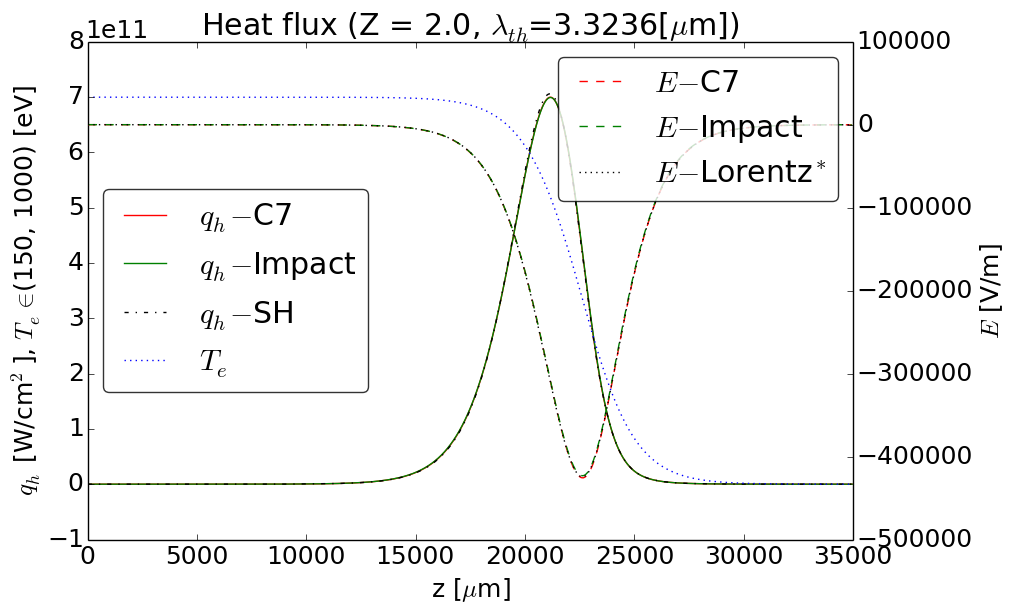
\includegraphics[width=\figscale\textwidth]{../VFPdata/C7_Impact_case1_heatflux.png} &
      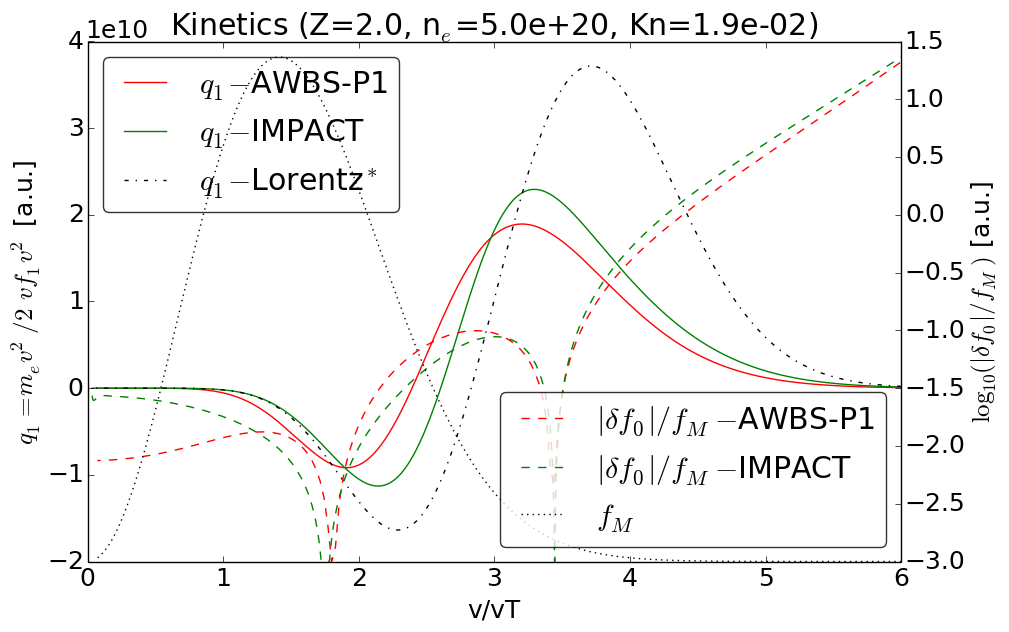
\includegraphics[width=\figscale\textwidth]{../VFPdata/C7_Impact_case1_kinetics.png}
    \end{tabular}
  \caption{  
  Impact diffusive case 1.}
  \end{center}
  \label{fig:C7_Impact_case1}
\end{figure}

\begin{figure}[tbh]
  \begin{center}
    \begin{tabular}{cc}
      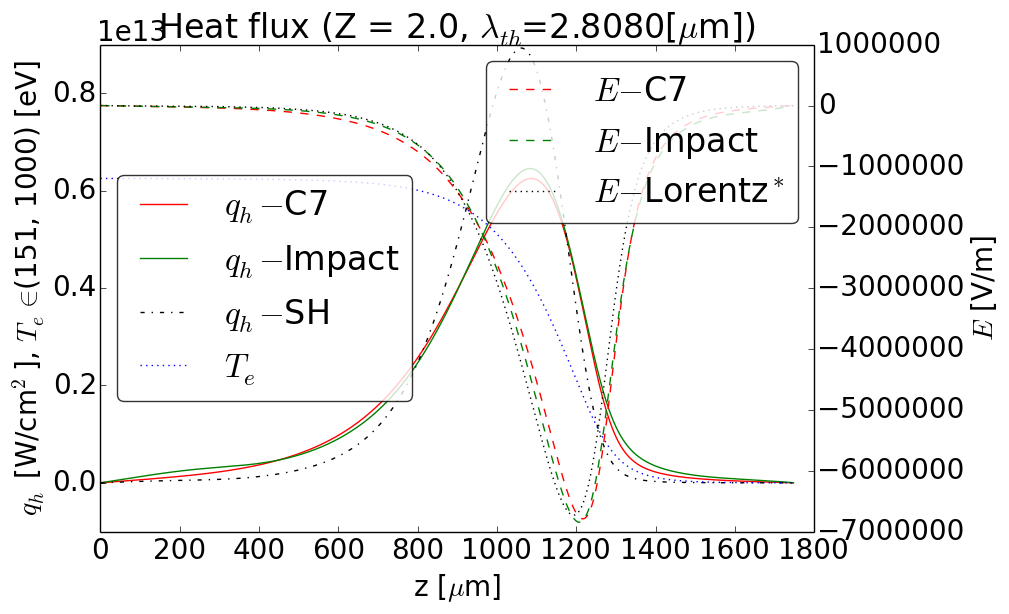
\includegraphics[width=\figscale\textwidth]{../VFPdata/C7_Impact_case2_heatflux.png} &
      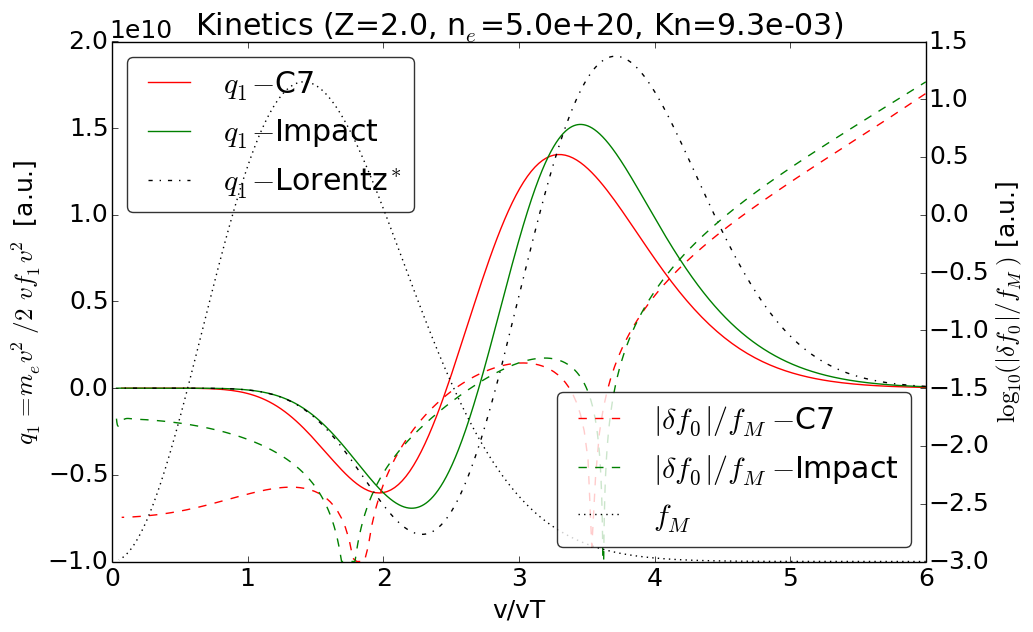
\includegraphics[width=\figscale\textwidth]{../VFPdata/C7_Impact_case2_kinetics.png}
    \end{tabular}
  \caption{  
  Impact case 2.}
  \end{center}
  \label{fig:C7_Impact_case2}
\end{figure}

\begin{figure}[tbh]
  \begin{center}
    \begin{tabular}{cc}
      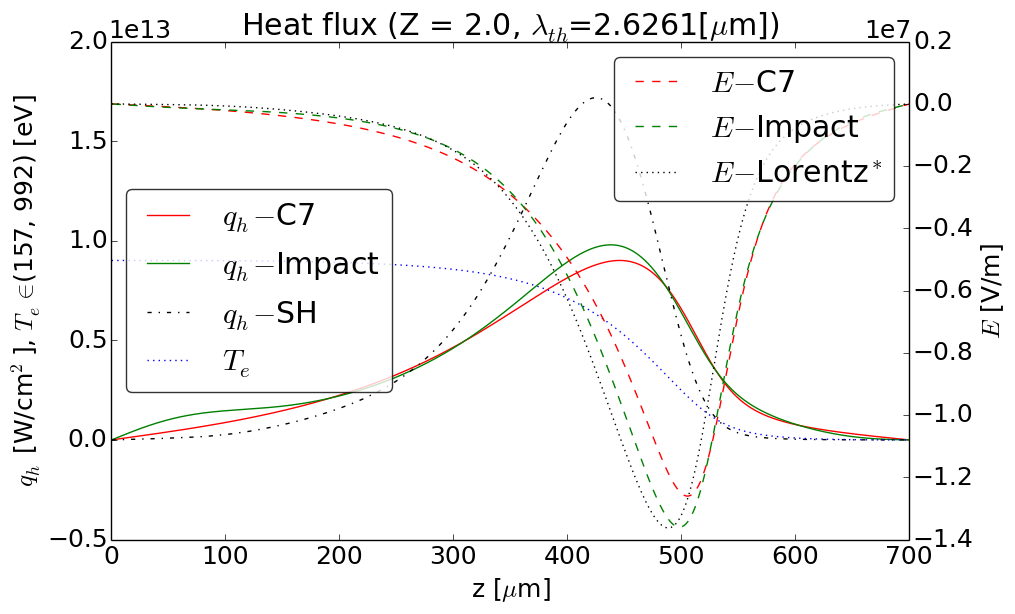
\includegraphics[width=\figscale\textwidth]{../VFPdata/C7_Impact_case3_heatflux.png} &
      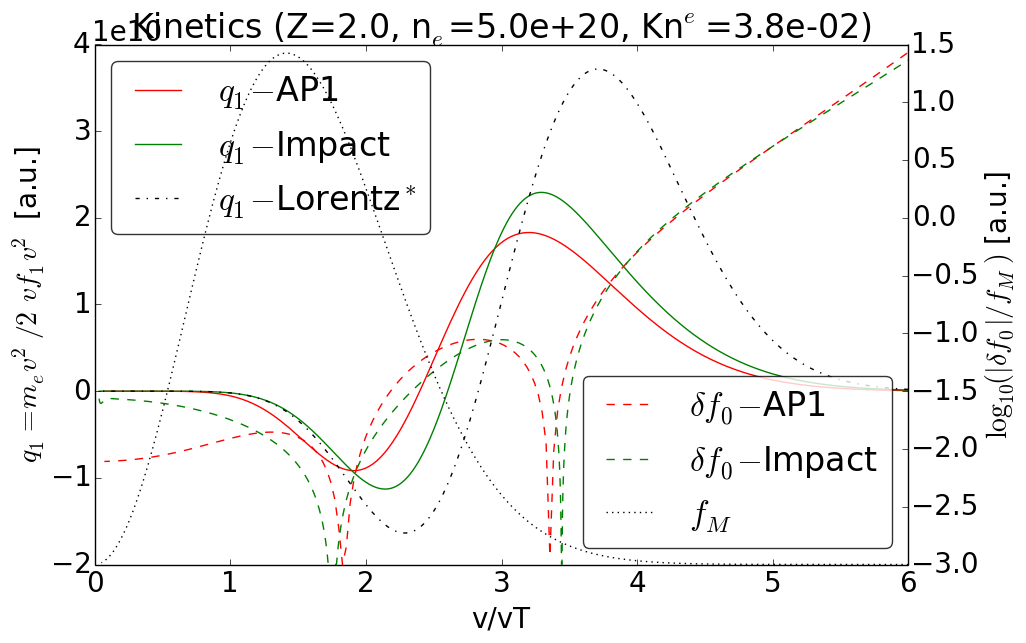
\includegraphics[width=\figscale\textwidth]{../VFPdata/C7_Impact_case3_kinetics.png}
    \end{tabular}
  \caption{  
  Snapshot 12 ps. Left: correct steady solution of heat flux. Right: correct comparison to kinetic profiles at point 437 $\mu$m by Impact.}
  \end{center}
  \label{fig:C7_Impact_case3}
\end{figure}

\begin{figure}[tbh]
  \begin{center}
    \begin{tabular}{cc}
      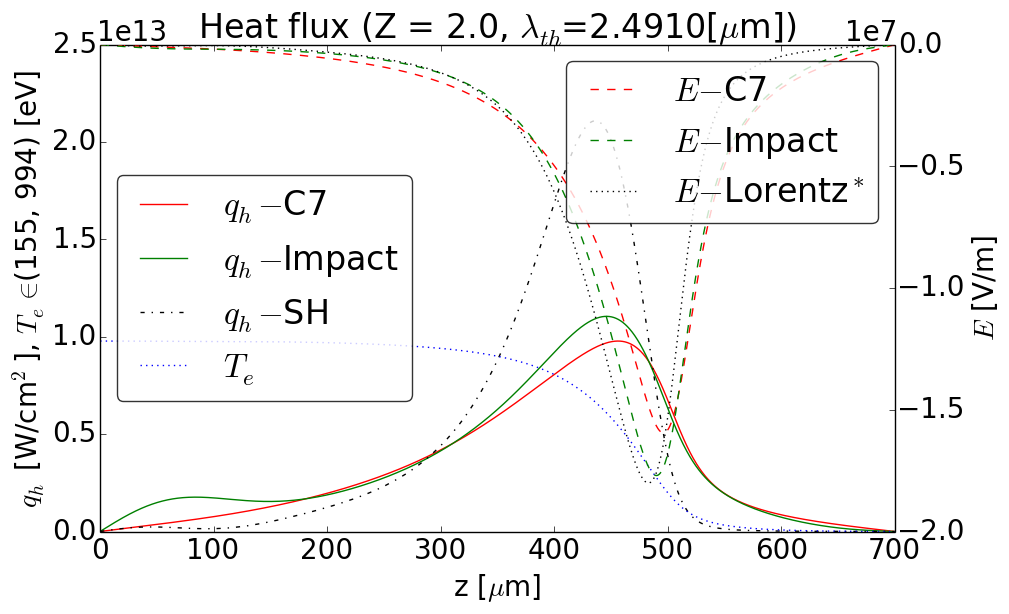
\includegraphics[width=\figscale\textwidth]{../VFPdata/C7_Impact_case4_heatflux.png} &
      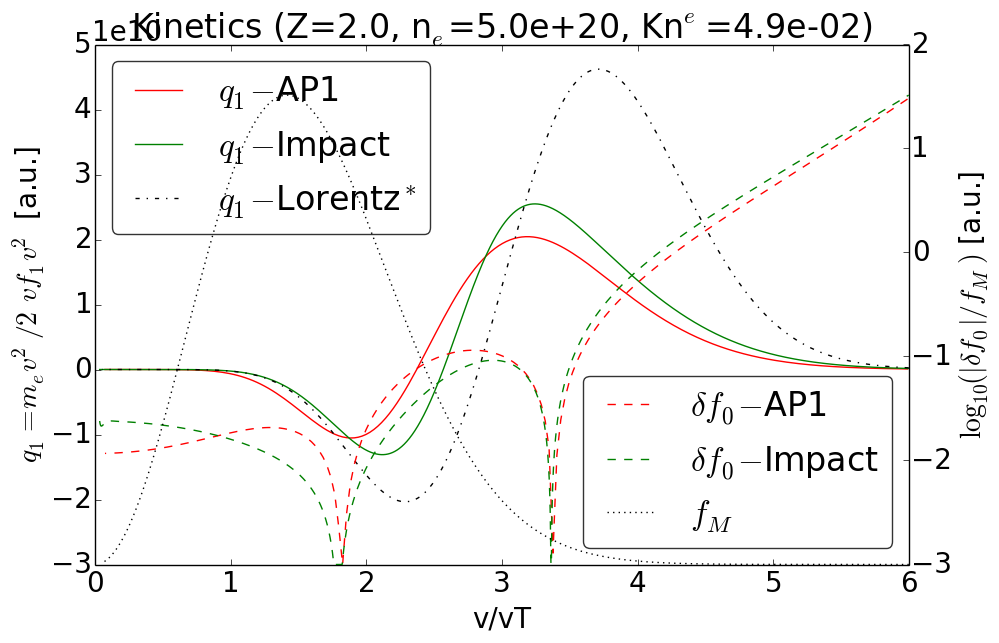
\includegraphics[width=\figscale\textwidth]{../VFPdata/C7_Impact_case4_kinetics.png}
    \end{tabular}
  \caption{  
  Impact case 4.}
  \end{center}
  \label{fig:C7_Impact_case4}
\end{figure}

\begin{figure}[tbh]
  \begin{center}
    \begin{tabular}{cc}
      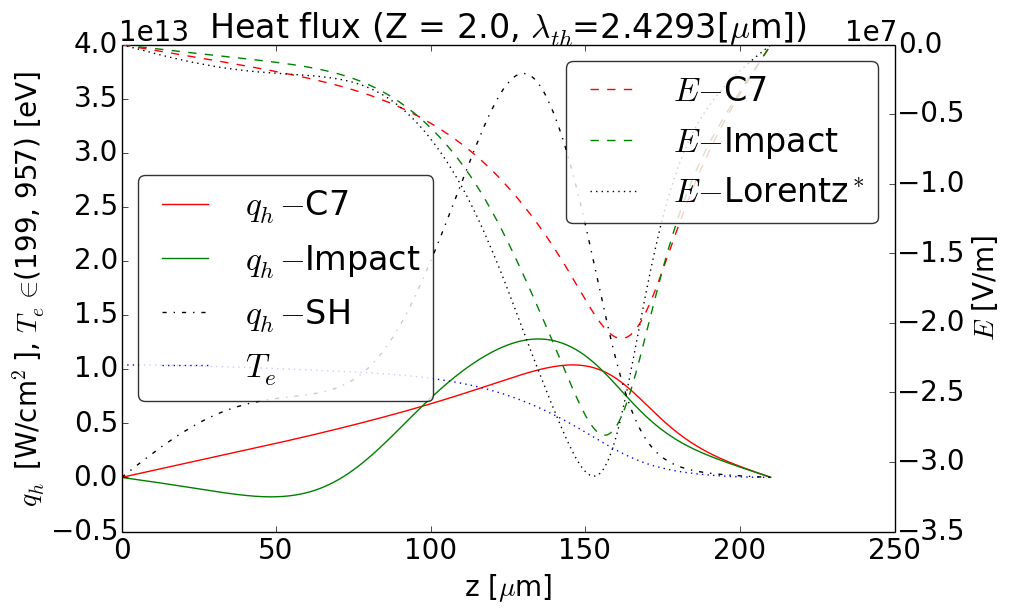
\includegraphics[width=\figscale\textwidth]{../VFPdata/C7_Impact_case5_heatflux.png} &
      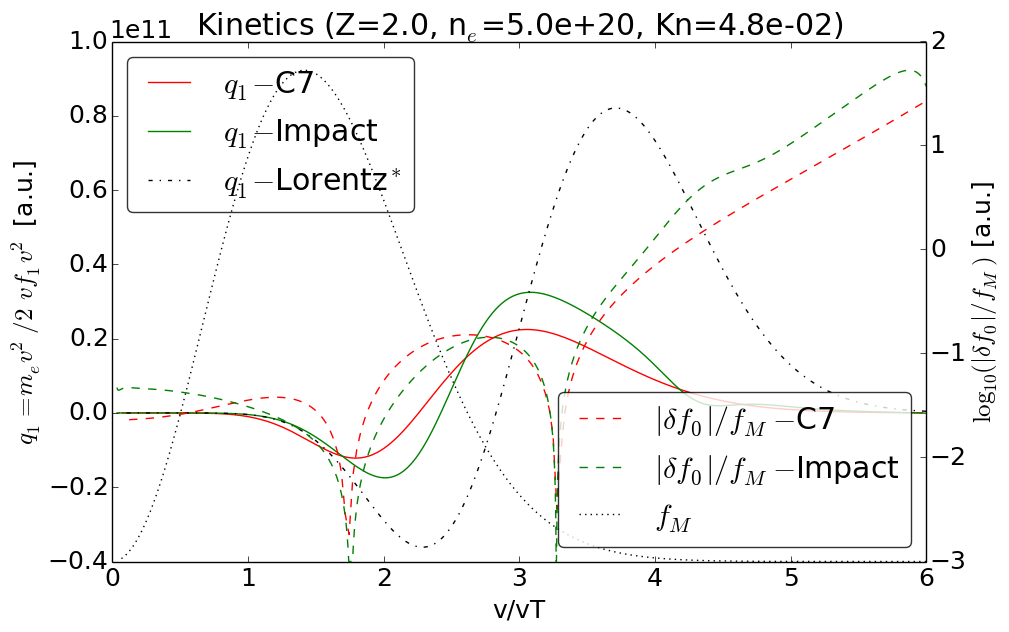
\includegraphics[width=\figscale\textwidth]{../VFPdata/C7_Impact_case5_kinetics.png}
    \end{tabular}
  \caption{  
  Impact case 5.}
  \end{center}
  \label{fig:C7_Impact_case1}
\end{figure}
\clearpage
%\end{comment} % All Impact figs
